\documentclass[12pt,a4paper]{article}
\usepackage[T1]{fontenc}
\usepackage[utf8]{inputenc}
\usepackage[margin=25mm]{geometry}
\usepackage{lmodern}
\usepackage{setspace}
\usepackage{lineno}
\usepackage{graphicx}
\usepackage{array,longtable,booktabs}
\usepackage[numbers,sort&compress]{natbib}
\usepackage[hidelinks]{hyperref}
\usepackage{amsmath,amssymb}
\setlength{\parindent}{0pt}
\setlength{\parskip}{6pt}
\setlength{\emergencystretch}{3em}
\setcounter{secnumdepth}{0}
\doublespacing
\renewcommand{\topfraction}{0.9}
\renewcommand{\bottomfraction}{0.85}
\renewcommand{\textfraction}{0.05}
\pagestyle{plain}
\begin{document}
\renewcommand{\thefigure}{S\arabic{figure}}\renewcommand{\thetable}{S\arabic{table}}\title{Supplementary methods and analyses for BINDRA}
\author{\normalsize Kevin Song, John Zhang, Lei Ye, and Jianyi Zhang}
\date{}
\begin{singlespace}\maketitle\end{singlespace}
\linenumbers
\section*{Supplementary protocol details}
This supplement describes the primary pooled BINDRA ensemble (C-matched) and the retained BINDRA-iBAM ensemble without FiLM (F). Each ensemble averages predictions in pKd space. Affinity weights remained fixed throughout the supporting analyses. Both ensembles use member seeds 20261001, 20261002, and 20261003.

\subsection*{Dataset identity and scope}
The official warm test contains 5010 pairs, with rows sorted by released pair index rather than the arbitrary order within the test-fold list. Fold membership and labels remain unchanged. The fitting/validation allocation uses official folds 1 through 4 and fold 0, respectively. All five training folds enter fixed-duration refits. Three-seed replication is not five-fold cross-validation.

The cold-drug split separates normalized chemical identities and excludes 884 rows identified by the identity/parent leakage audit. This separation does not establish scaffold novelty. The cold-protein split excludes exact sequence identities, not all homologous proteins. Separate ensembles were trained for these protocols. Similarity to the nearest training molecule or sequence describes the degree of novelty. Calibration was withheld because full-pool warm models lacked independent calibration observations, while normalized-pair duplication required stronger separation in the cold protocols.

Earlier Davis experiments with adapted encoders included test inspection. Subsequent validation-based architecture selection does not restore an untouched test set. All eight warm-arm validation records and all executed individual-model metrics are supplied, including unsuccessful variants. The controlled experiments used the original frozen ESM-C and five-epoch ligand checkpoints; models with historical encoder adaptation were analyzed separately.

\subsection*{Metric definitions}
For measured pKd y and prediction p, MSE is the mean of (y - p) squared, RMSE is its square root, and MAE is the mean absolute difference. CI averages correct-order credit over unequal measured-label pairs, with one-half credit for prediction ties. Within-target macro CI is the unweighted mean over target sequences with comparable pairs. It is distinct from pooled CI and from a mean weighted by target-pair counts.

For the \(r_m^2\) diagnostics, define r2 as squared Pearson correlation and r02 as the zero-intercept fit coefficient in the measured-label direction. The conventional diagnostic is r2 multiplied by (1 - sqrt(abs(r2 - r02))). The DeepDTA implementation instead uses r2 multiplied by (1 - sqrt(abs(r2 squared - r02 squared))). Both are exported under explicit names, with the exact implementation in the source snapshot. The two definitions are not interchangeable.

The active threshold is measured pKd \(\geq\) 7. Average precision is the recall-increment-weighted mean of precision. Trapezoidal precision-recall area uses linear interpolation between the computed precision-recall points. They are separate metrics. Equivalence to the historical auc.jar integration was not established. For a candidate pool of size N and active count A, EF1\% is (a/k)/(A/N), where k is max(1, ceiling(0.01N)) and a is the active count in the top k candidates. Recall@k is the recovered active fraction using min(k, N) candidates. Therefore, Recall@100 can be one in a pool with fewer than 100 candidates without demonstrating strong early enrichment.

Crossed bootstrap intervals resample exact construct-sequence and Murcko-scaffold groups, retain the product of group resampling weights, and use common weights in paired model comparisons. The warm contrast includes 379 sequence groups and 68 Murcko-series groups. These resampling units do not capture all dependence within protein families or chemical series. The F-minus-C-matched warm MSE-difference interval spans -0.01464 to 0.01410. Seed standard deviations describe variation between fitted runs and are not these bootstrap intervals. No significance test is performed against literature point values.

\subsection*{Literature provenance and comparability}
The numerical registry covers literature through October 17, 2026; bibliographic metadata were checked during manuscript preparation. The literature-only CSV excludes the historical adapted BINDRA row while preserving the original source. Registry statements about BINDRA five-fold selection refer to historical experiments; the controlled study used one validation fold.

The DeepDTA and released GraphDTA fold files were verified directly. However, the upstream GraphDTA training script permits test-based checkpoint selection, which limits comparability. WideDTA, MGraphDTA, and DeepDTAGen claim canonical-style folds without independent observation-hash equivalence. FusionDTA aggregation and exact selection were not fully verified. NHGNN-DTA used an 80/10/10 random split with 3006 test pairs, and SSM-DTA used a 70/10/20 split. Predicted protein contacts, binding-site supervision, and affinity-derived graphs are additional inputs or supervision, even when inference begins with sequences and SMILES. Results from unverified protocols are not treated as matched comparisons.

\nolinenumbers\begin{table}[htbp]\centering\begin{singlespace}\small\setlength{\tabcolsep}{3pt}\renewcommand{\arraystretch}{1.3}
\caption{Author-reported Davis results for all reviewed model variants}
\begin{tabular}{>{\raggedright\arraybackslash}p{0.35\linewidth}>{\raggedright\arraybackslash}p{0.08\linewidth}>{\raggedright\arraybackslash}p{0.1\linewidth}>{\raggedright\arraybackslash}p{0.1\linewidth}>{\raggedright\arraybackslash}p{0.23\linewidth}}
\toprule
\textbf{Method} & \textbf{Year} & \textbf{MSE} & \textbf{CI} & \textbf{Qualification}\\\midrule
DeepDTA \citep{deepdta2018} & 2018 & 0.261 & 0.878 & A\\
WideDTA \citep{widedta2019} & 2019 & 0.262 & 0.886 & B\\
DGraphDTA \citep{dgraph2020} & 2020 & 0.202 & 0.904 & C\\
GraphDTA (GAT) \citep{graphdta2021} & 2021 & 0.232 & 0.892 & A\\
GraphDTA (GAT\_GCN) \citep{graphdta2021} & 2021 & 0.245 & 0.881 & A\\
GraphDTA (GCN) \citep{graphdta2021} & 2021 & 0.254 & 0.880 & A\\
GraphDTA (GIN) \citep{graphdta2021} & 2021 & 0.229 & 0.893 & A\\
FusionDTA \citep{fusion2022} & 2022 & 0.208 & 0.913 & B\\
FusionDTA (KD, large) \citep{fusion2022} & 2022 & 0.205 & 0.914 & B\\
MGraphDTA \citep{mgraph2022} & 2022 & 0.207 & 0.900 & B\\
MFR-DTA \citep{mfr2023} & 2023 & 0.221 & 0.905 & C\\
NHGNN-DTA \citep{nhgnn2023} & 2023 & 0.196 & 0.914 & D1\\
SSM-DTA \citep{ssm2023} & 2023 & 0.219 & 0.890 & D2\\
HGTDP-DTA \citep{hgtdp2024} & 2024 & 0.142 & 0.910 & C, preprint\\
MDF-DTA \citep{mdf2024} & 2024 & 0.172 & 0.912 & C\\
ProSmith \citep{prosmith2024} & 2024 & 0.186 & 0.911 & D1\\
DeepDTAGen \citep{deepdtagen2025} & 2025 & 0.214 & 0.890 & B\\
HCAF-DTA \citep{hcaf2025} & 2025 & 0.198 & 0.908 & C, preprint\\
CurvFlow-DTA \citep{curvflow2026} & 2026 & 0.185 & 0.902 & C, preprint\\
\bottomrule\end{tabular}\par\vspace{6pt}
{\raggedright\footnotesize All 19 values are author-reported, not local reruns. A: official fold files verified, selection and aggregation qualified; the released GraphDTA training script includes test-based selection. B: exact fold identity, selection or aggregation not fully verified; WideDTA is a preprint version. C: additional structural inputs, binding-site supervision or affinity-derived graphs; not input-matched. D1: alternate random 80/10/10 settings. D2: random 70/10/20 split. Exact split and resource differences are detailed in the source-linked registry. Preprint labels refer to the versions reviewed. BINDRA uses external pretraining and prediction averaging; no cross-paper significance or universal superiority claim is made.\par}
\end{singlespace}\end{table}
\linenumbers
\section*{Structural mappings and controls}
Complexes were selected by structural quality and target coverage. Each of the 30 complexes has a chemical mapping and construct-to-author residue map, including missing-residue and insertion-code handling. Eligibility requires a noncovalent small-molecule complex, resolution \(\leq\) 2.5 angstrom, usable coordinates, and unambiguous sequence/chemical correspondence. At most three complexes represent any target group. The final panel has ten target groups and no selection shortfall.

For each member, last-layer attention is averaged over heads. Member maps are combined only after residue and ligand coordinates are aligned. Individual heads, both attention directions, and knowledge-token mass remain available. Contact scores use physical tokens and resolved residues. Primary contacts were defined by a minimum heavy-atom distance \(\leq\) 4 angstrom, with sensitivity analyses at 3.5 and 5 angstrom. A large residue AP can coexist with poor residue-atom or ligand-atom agreement; those outcomes remain separate.

Contact prevalence and residue-score permutations provide reference values. Target-group bootstrap intervals equally weight the ten target groups. Head/member agreement, representation reordering, progressive parameter randomization, swaps in predictions, and protein-feature gradients assess different aspects of model behavior. Ten matched random masks accompany 10\% residue-feature masks. These are feature perturbations, not physical mutations, and can be outside the training distribution. Integrated gradients, additional masking fractions, and coordinate-aligned explanation-map swaps were not evaluated.

\subsection*{FAK1 and P4N}
PDB 6YOJ supplies the detailed FAK1-P4N structural illustration at 1.361-angstrom resolution. Residue indices in the numeric exports map to PDB author numbering. Min-max displays, where used, are explicitly labeled and accompanied by raw weights. BINDRA-iBAM predicted a pKd of 5.41667 for this input. Ki and IC50 source annotations remain assay-qualified and are not treated as trained prediction endpoints or numerically interchangeable pKd labels.

The complete Kd inventory for the focal construct contains 12 unique ligands, including three actives, four weak compounds, and five intermediate/discordant cases. The seven-compound active/weak subset falls below the primary screening coverage requirement and was analyzed as an exploratory example alongside the eligible measured-negative panels.

The main-text case figure shows the raw physical-token iBAM alongside ligand-only bond attention and a protein-to-ligand bond marginal. These matrices have different query/key axes and normalization domains. For 6YOJ, residue AP was 0.17648, but derived residue-atom AP was 0.04178 for ligand-to-protein attention and 0.00785 for protein-to-ligand attention, against contact prevalence 0.00784. Thus, residue-level correspondence did not imply equally informative pairwise localization in both directions. Moreover, 31 of 34 ligand heavy atoms contacted the protein, giving atom-contact prevalence 0.91176. Ligand-atom AP was 0.86535 for ligand-to-protein attention and 0.85919 for protein-to-ligand attention, below that reference. These single-complex diagnostics do not support an atom-level contact-recovery claim. The full matrices, mapped author residue numbers, and physical-token mappings accompany the case figure; min-max display scaling, where used, is separate from quantitative scoring.

\begin{figure}[htbp]\centering
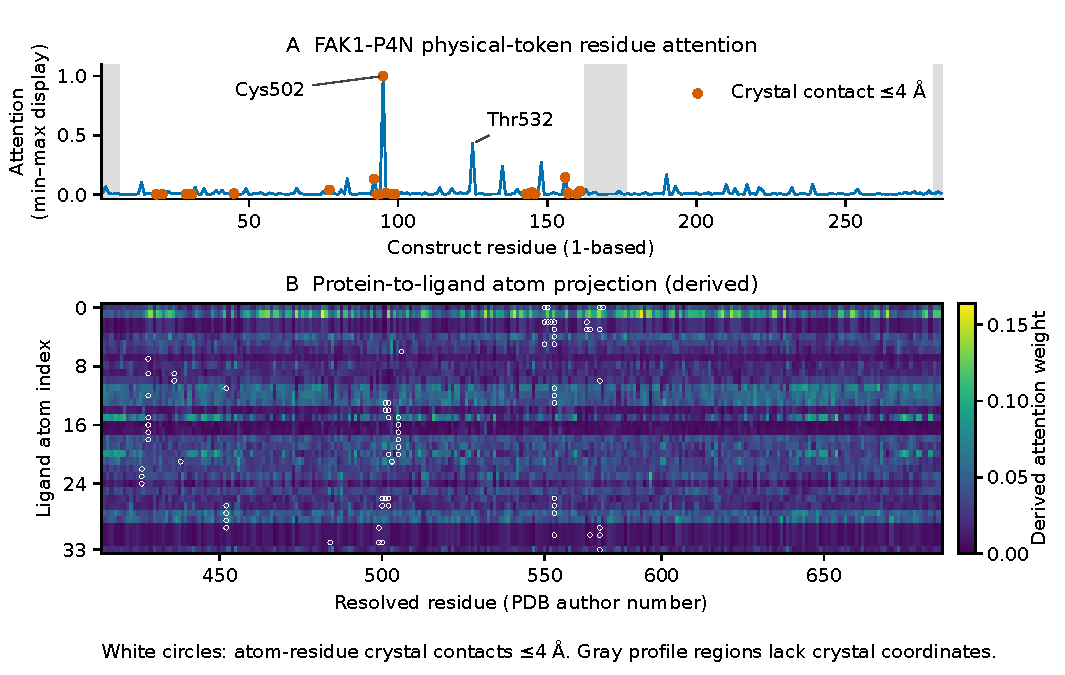
\includegraphics[width=\linewidth,height=.65\textheight,keepaspectratio]{figures/Supplementary_Figure_1_FAK_contacts.pdf}
\caption{FAK1-P4N physical-token attention and derived atom projection. PDB 6YOJ, at 1.361-angstrom resolution, has 259 resolved residues within the 282-residue modeled construct. The upper profile averages ligand-to-protein attention over 37 physical bond tokens and is min-max scaled only for display; gray regions lack crystal coordinates. Contact residues use the 4-angstrom cutoff. The lower panel is a derived protein-to-ligand atom projection: each bond-token weight is divided equally between its mapped endpoint atoms. White circles mark crystal atom-residue contacts. This projection is not native atom-level attention. PDB author numbering and unscaled weights are exported; no display scaling enters contact scoring.}
\end{figure}
\begin{figure}[htbp]\centering
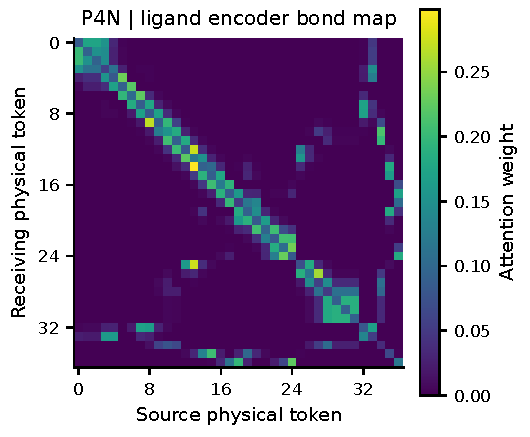
\includegraphics[width=\linewidth,height=.65\textheight,keepaspectratio]{figures/Supplementary_Figure_2_FAK_bonds.pdf}
\caption{P4N ligand-only bond attention. The heatmap shows attention between physical ligand tokens in the shared frozen LiGhT-mini encoder, before protein conditioning. Rows are receiving tokens and columns are source tokens; weights are unitless. Knowledge tokens are excluded from this physical-token display, and their attention mass is exported separately. The map is target independent and shared by the affinity members; it does not establish physical interactions between bonds.}
\end{figure}
\subsection*{Bond attention is a shared ligand representation}
Bond maps are computed before target conditioning. The three affinity members share one frozen ligand encoder, so repeated member maps are not independent encoder replications. Controls summarize 27 unique ligands in 25 chemical components. Full-matrix and supported-edge correlations are labeled separately; the latter were added after inspecting full-matrix behavior and are secondary analyses. Atom-order sensitivity and persistence under layer randomization are limitations. Whole-encoder randomization generally produces larger map changes. The exports include topology controls, symmetry-aware atom/bond mappings, knowledge-token mass, and mapped analog edits.

\begin{figure}[htbp]\centering
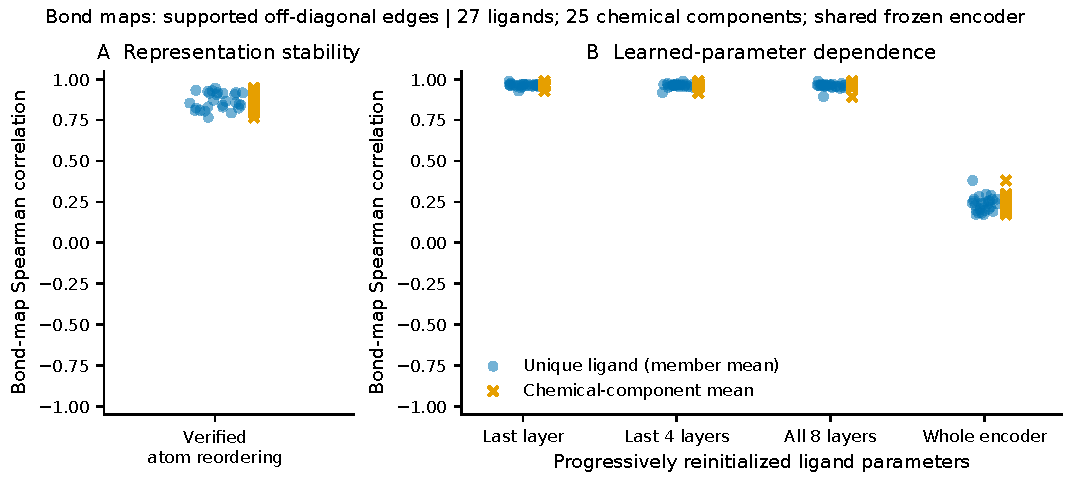
\includegraphics[width=\linewidth,height=.65\textheight,keepaspectratio]{figures/Supplementary_Figure_3_bond_controls.pdf}
\caption{Ligand bond-map sensitivity controls. Controls cover 27 unique ligands in 25 connected chemical groups. This figure evaluates mapped, supported off-diagonal attention entries. Panel A assesses atom-order stability, and panel B progressively randomizes ligand-encoder parameters. Points show per-ligand summaries; crosses show chemical-group means. The shared ligand encoder is not three independent replicates. Full-matrix results are reported separately; agreement under randomization limits interpretation as a learned chemical explanation.}
\end{figure}
\section*{Screening interpretation}
Measured weak compounds require exact eligible Kd observations at pKd \(\leq\) 5, and actives require pKd \(\geq\) 7. Intermediate and discordant measurements remain outside the binary measured subset. Presumed decoys were not assigned measured affinity labels. Full pools contain 1348 galectin-3, 329 beta-2 adrenergic receptor, and 227 KEAP1 candidates; measured subsets contain 73, 25, and 38. The decoy shortfalls are zero, 21, and 111, respectively.

For both ensembles, exports include target-only predictions, seed-assisted percentile-rank averaging, fingerprint similarity, property similarity, and a fixed random ranking. Seed-assisted methods receive information not supplied to the target-only predictor. Chemical-component bootstrap units use transitive identity, parent, and scaffold connections. Some bootstrap resamples contain only one class; interval summaries therefore report the number of finite resamples. Small numbers of components can make these intervals unstable. The three panels are outside the kinase-focused Davis target domain, and no general screening benefit is inferred from them.

\section*{Generator data and evaluation}
The raw cohort contains 93454 directed source edits across fitting and validation. Graph quality control retains 41682 fitting and 24819 validation edits and exports 26953 exclusions. Related molecules, reverse edits, and connected chemical series remain together. Each series contributes at most 32 directed pairs. Product graphs provide denoising targets, not conditioning features. Cached target and seed features are bound to the frozen BINDRA-iBAM ensemble. Each member's learned feature space is retained separately.

Six conditions each use three training seeds. Structured context uses actual mapped seed-atom iBAM information. Uniform context removes localization while retaining the context interface; shuffled context permutes atom-to-context assignments without changing atom identity. Global-only removes local attention context. Seed-only removes all target-derived features, including target length. Target-shuffled substitutes a different target using a fixed permutation. Capacity and draw budgets are matched.

Requested-delta support would require source-verified same-assay training groups with at least 20 undirected edits, ten molecules, and three series, within the training fifth-to-95th-percentile delta range. No group qualifies, so requested-delta conditioning is disabled. Proxy assay context does not establish measured potency improvement.

Every query/run exports 100 draws and a completion manifest. Raw validity requires a supported chemical reconstruction under the recorded sampling policy. No repair was applied, so repaired validity cannot exceed raw validity. Uniqueness is the number of unique valid chemical identities divided by the number of valid draws within a query/run. Scaffold retention is reported over all draws. Recovery compares generated identities with eligible held-out measured analog identities; it is not a predicted-score improvement. Novelty against generator training, ligand pretraining, and Davis supervision is reported separately.

The strict Kd subset has five queries across three series, generating 9000 draws across six conditions and three seeds. All conditions have 100\% validity and scaffold retention and zero measured-analog recovery. The broader 50-query set adds 18 Ki and 27 IC50 queries. The structured arm's 88.37\% overall raw validity is an equal-query/equal-seed mean, whereas bootstrap interval centers in the summary table equally weight chemical series. These weighting schemes summarize different quantities and are reported separately. Absence from a specified reference set does not establish novelty across public chemistry.

\section*{Native and generated docking}
Native redocking uses three seeds and exhaustiveness 32 with the same preparation and search settings across comparisons. A receptor must have at least two top-ranked poses with symmetry-aware RMSD \(\leq\) 2 angstrom and acceptable pose checks. The unsuccessful 5Y80 redocking result is retained. FAK1 has no eligible held-out generator query, and the generated analysis covers only the qualifying 9F3V-associated query.

\begin{singlespace}\small\setlength{\tabcolsep}{3pt}\begin{longtable}{p{.12\linewidth}p{.13\linewidth}p{.40\linewidth}p{.12\linewidth}p{.12\linewidth}}
\caption{Native redocking outcomes across search seeds}\\\toprule PDB & Ligand & Top-pose RMSD in seed order (angstrom) & Pose checks & Qualified\\\midrule
6YOJ & P4N & 0.385/0.371/0.361 & 3/3 & True\\
5Y80 & IRE & 3.858/3.935/3.891 & 0/3 & False\\
9F3V & A1H90 & 11.318/1.098/1.165 & 2/3 & True\\
\bottomrule\end{longtable}\end{singlespace}
\begin{figure}[htbp]\centering
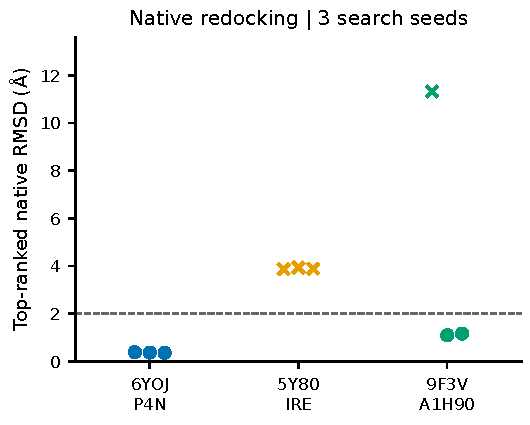
\includegraphics[width=\linewidth,height=.65\textheight,keepaspectratio]{figures/Supplementary_Figure_4_native_docking.pdf}
\caption{Native-ligand redocking by receptor and search seed. Three search seeds per receptor used exhaustiveness 32. Points show symmetry-aware heavy-atom RMSD for the top-ranked native-ligand pose in the experimental receptor frame; the dashed line marks 2 angstrom. A receptor qualifies only when RMSD is at most 2 angstrom and pose checks pass in at least two seeds. 6YOJ qualified in three seeds, 9F3V in two, and 5Y80 in none. Failed redocking remains reported.}
\end{figure}
The 90 generated selections represent compound instances within each query, condition, and training-seed run. Fifty-five fail preparation and 35 yield 105 repeated-search poses, with 91 passing overall PoseBusters checks. The selection policy is hash-based and independent of affinity or docking scores. The pose pass rate is conditional on successful preparation; its denominator excludes preparation failures. Preparation failures, stereochemistry/geometry checks, and search outputs are retained. Docking scores describe computed poses and do not measure binding or potency.

\section*{Reproducibility and data availability}
The read-only reproducibility checker verifies frozen member hashes, official fold membership, ensemble arithmetic, numerical metrics, table provenance, all 18 generator checkpoint/sample identities, and figure export requirements. Source code, environment, optimizer, exponential moving average (EMA), and random-number-generator (RNG) records support resumption under matching settings. Inductor/Triton acceleration was retained only where numerical checks passed; batch-conditioning acceleration that failed these checks was rejected.

The additional files contain machine-readable results and all generated-draw records. The complete 4.35-GB research archive is retained separately. Checkpoints, original per-head arrays, full chemical SDF exports, and licensed third-party assets require an appropriate repository and access/licensing statement. The local checksum inventory identifies these assets. The paper remains a submission draft until the authors confirm contribution roles, funder involvement, acknowledgments, exclusive-submission/originality statements, approval, and persistent code/data identifiers.

\section*{Detailed supporting methods and results}
\subsection*{Retrospective compound fishing}
We froze target eligibility, candidate pools, seeds, ranking rules, and exposure audits before scoring. Primary measured-negative pools required at least ten actives at pKd \(\geq\) 7 and ten weak compounds at pKd \(\leq\) 5 after seed exclusion. Intermediate or discordant measurements were not converted to negative labels. Three eligible construct panels mapped to galectin-3 (P17931), beta-2 adrenergic receptor (P07550), and KEAP1 (Q14145). Exact sequences and normalized chemical identifiers accompany the source tables.

Each candidate was scored exhaustively by both frozen ensembles. Target-only pKd rankings were compared with Morgan fingerprint similarity to the seed, standardized property similarity, a fixed random ranking, and seed-assisted retrieval. Seed-assisted retrieval equally averaged full-pool pKd and similarity percentile ranks. Seed-assisted methods were identified as receiving additional information. Exact seeds and duplicate chemical identities were removed. Unlabeled compounds were not assigned measured affinity labels.

Measured weak compounds and property-matched presumed decoys were analyzed separately. The decoy target was 25 per active, with shortfalls retained. Metrics included full-pool EF1\%, AP, Recall@10, Recall@50, Recall@100, candidate counts, and prevalence. Chemical-component bootstrap intervals preserved related compounds, with the number of finite resamples reported when a resample lacked both classes. FAK1's measured Kd pool did not meet the primary coverage requirement and remained exploratory.

\subsection*{Independent analog generation}
We built endpoint-labeled analog edits from exact measurements with compatible protein constructs and available assay context. Chemical series, shared molecules, reverse pairs, and related edits remained together across partitions. Each series contributed at most 32 directed pairs, selected deterministically. Exposed evaluation components and graph failures were excluded and recorded. Source-verified assay groups were distinguished from proxy comparability groups; the latter do not establish measured potency improvements.

The diffusion generator had separate parameters, optimizer, exponential moving average, and random-number-generator state. The entire BINDRA-iBAM ensemble remained frozen. Conditioning used the actual seed graph and tokens, endpoint, target residue features, member-specific fusion features, and seed-atom-aligned iBAM context. Generator-owned projections retained each member's feature space separately. Conditioning excluded product-derived features. Requested-delta conditioning was disabled because no source-verified same-assay groups met the training-support criteria.

The compact generator used dimension 128, three layers, four attention heads, a 64-atom cap, 500 forward diffusion steps, and 100 exact-posterior reverse evaluations. Target features were pooled to 32 residue tokens per member. Training used batch size 64, learning rate 0.0001, weight decay 0.01, at most 20 epochs, and patience three. Endpoint- and series-balanced validation denoising loss selected checkpoints. Six capacity-matched conditions were trained with three seeds each: structured iBAM, global-only, uniform iBAM, shuffled iBAM, seed-only, and target-shuffled. Seed-only removed all target-derived information. Shuffling changed seed-atom-to-context assignments rather than atom identities.

We selected 50 eligible held-out queries without using model performance: five strict Davis-construct Kd queries across three chemical series, followed by 18 Ki and 27 IC50 queries allocated by endpoint and target coverage. Every query received 100 draws per condition and seed. Evaluation included raw validity, uniqueness among valid molecules within a query/run, scaffold retention, seed-copy rate, diversity, seed similarity, and measured-analog recovery. Novelty against generator training, ligand pretraining, and Davis supervision was assessed separately using the declared chemical-identity normalization. Supported scaffold stereochemistry was preserved, unspecified new centers were flagged, and repair was disabled. Affinity-model scores were outside generator optimization.

\subsection*{Bounded docking assessment}
We used AutoDock Vina 1.2.7, Meeko 0.8.0, and PoseBusters 0.6.5 \citep{vina2021,meeko,posebusters2024}. Native redocking used three search seeds and exhaustiveness 32. A receptor qualified if the top-ranked pose had symmetry-aware heavy-atom root-mean-square deviation (RMSD) \(\leq\) 2 angstrom and passed pose checks in at least two seeds. Ligands were compared in the experimental receptor frame, not superimposed independently to remove pose error.

Generated-compound docking was restricted to qualifying receptors with eligible held-out Kd queries. Up to five valid, unique, generator-training-novel compounds per query, condition, and training seed were selected by hash, not affinity or docking score. Preparation failures, poses, geometry checks, and docking scores were retained. Pose-level checks were conditional on successful preparation and repeated search poses were not independent compounds. No docking result was interpreted as experimental binding confirmation.

\subsection*{Retrospective screening did not establish general ranking superiority}
The three measured-negative panels contained 73, 25, and 38 candidates after filtering, with active prevalences 0.699, 0.520, and 0.316. Their full pools with presumed decoys contained 1348, 329, and 227 candidates, respectively. Two pools fell short of the requested decoy ratio, by 21 and 111 compounds; these shortfalls were retained.

On the measured panels, primary BINDRA AP was 0.533, 0.408, and 0.487 for galectin-3, beta-2 adrenergic receptor, and KEAP1. BINDRA-iBAM achieved 0.681, 0.513, and 0.324. Fingerprint similarity achieved 0.983, 0.920, and 0.720. Seed-assisted retrieval improved some model rankings but did not establish consistent superiority over similarity or property controls (supplementary screening table). Similarity and property controls received a known active seed, whereas target-only prediction did not. Results are labeled by the information supplied to each method.

These panels lie outside the kinase-focused Davis training domain and do not establish broadly calibrated affinity prediction. Full-pool EF1\%, recall, candidate labels, exposure strata, and chemical-component intervals, including unstable or nonfinite resamples, are retained in Additional file 2. FAK1 was retained as an exploratory case alongside all eligible screening panels.

\nolinenumbers\begin{table}[htbp]\centering\begin{singlespace}\small\setlength{\tabcolsep}{3pt}\renewcommand{\arraystretch}{1.3}
\caption{Measured-negative screening average precision}
\begin{tabular}{>{\raggedright\arraybackslash}p{0.2621276595744681\linewidth}>{\raggedright\arraybackslash}p{0.05617021276595744\linewidth}>{\raggedright\arraybackslash}p{0.09361702127659575\linewidth}>{\raggedright\arraybackslash}p{0.12170212765957446\linewidth}>{\raggedright\arraybackslash}p{0.12170212765957446\linewidth}>{\raggedright\arraybackslash}p{0.11234042553191488\linewidth}>{\raggedright\arraybackslash}p{0.11234042553191488\linewidth}}
\toprule
\textbf{Target} & \textbf{N} & \textbf{Actives} & \textbf{Active fraction} & \textbf{BINDRA AP} & \textbf{iBAM AP} & \textbf{Seed FP AP}\\\midrule
Galectin-3 & 73 & 51 & 0.699 & 0.533 & 0.681 & 0.983\\
Beta-2 adrenergic receptor & 25 & 13 & 0.520 & 0.408 & 0.513 & 0.920\\
KEAP1 & 38 & 12 & 0.316 & 0.487 & 0.324 & 0.720\\
\bottomrule\end{tabular}\par\vspace{6pt}
{\raggedright\footnotesize AP is average precision, not trapezoidal PR-AUC. BINDRA and iBAM columns are target-only pKd rankings; the fingerprint method receives an active seed. Exact seeds and duplicate identities are removed. These retrospective non-kinase panels do not establish general screening superiority. Presumed decoys, seed-assisted/property/random methods, full-pool EF1\%, recall and chemical-component intervals remain in Additional file 2.\par}
\end{singlespace}\end{table}
\linenumbers
\subsection*{Valid generation did not translate into measured-analog recovery}
Graph quality control retained 41682 fitting and 24819 validation directed edits from 93454 source pairs. All 18 generator fits and 900 query/run evaluations completed, producing 90000 draws. Across all 50 queries, structured conditioning had equal-seed mean raw validity 88.37\%. In the primary five-query strict Kd subset, all six conditions achieved 100\% raw validity and scaffold retention without repair (supplementary generator table; supplementary generator figure). Structured within-query uniqueness was 99.27\% in this subset.

None of the six conditions recovered a held-out measured analog in the 9000 strict-Kd draws. All conditions therefore had zero recovery on the primary outcome. The structured condition's high validity and exact training-set novelty did not establish that target information improved biological design. Uniform and target-shuffled conditions could attain lower validation denoising losses than structured conditioning, reinforcing the distinction between optimizing a denoising objective and demonstrating useful conditional generation.

The strict subset contained five queries across only three chemical series, limiting target coverage. Zero recovery should therefore be interpreted within the available measured analogs and sampling budget. Ki and IC50 strata, novelty against each reference set, seed-copy rates, rejection reasons, diversity, and per-seed losses accompany the full exports. No generated compound was described as experimentally validated or as a measured potency improvement.

\nolinenumbers\begin{table}[htbp]\centering\begin{singlespace}\small\setlength{\tabcolsep}{3pt}\renewcommand{\arraystretch}{1.3}
\caption{Generator outcomes across conditioning controls}
\begin{tabular}{>{\raggedright\arraybackslash}p{0.225\linewidth}>{\raggedright\arraybackslash}p{0.16875\linewidth}>{\raggedright\arraybackslash}p{0.16875\linewidth}>{\raggedright\arraybackslash}p{0.16875\linewidth}>{\raggedright\arraybackslash}p{0.16875\linewidth}}
\toprule
\textbf{Condition} & \textbf{All-query validity (\%)} & \textbf{Strict-Kd validity (\%)} & \textbf{Strict-Kd uniqueness (\%)} & \textbf{Strict-Kd recovery (\%)}\\\midrule
Structured iBAM & 88.37 & 100.00 & 99.27 & 0.00\\
Global only & 88.90 & 100.00 & 99.00 & 0.00\\
Uniform iBAM & 88.26 & 100.00 & 99.33 & 0.00\\
Shuffled iBAM & 88.19 & 100.00 & 99.20 & 0.00\\
Seed only & 89.38 & 100.00 & 99.20 & 0.00\\
Target shuffled & 89.04 & 100.00 & 99.00 & 0.00\\
\bottomrule\end{tabular}\par\vspace{6pt}
{\raggedright\footnotesize Equal-query/equal-seed means; three seeds per condition and 100 draws/query/run. The full set has 50 queries and 90000 draws. Strict Kd has five queries, three chemical series and 9000 draws; scaffold retention is 100\% in every condition. Uniqueness is conditional on valid draws within a query/run. Repair is none. Endpoint/series intervals are separate exports; exact novelty does not establish public chemical novelty or binding.\par}
\end{singlespace}\end{table}
\linenumbers
\subsection*{Docking supported a narrow geometry assessment}
Native redocking qualified 6YOJ in three of three seeds and 9F3V in two of three; 5Y80 qualified in none. FAK1 had no eligible held-out generator query, so it contributed native redocking only. Generated docking was consequently limited to the qualifying 9F3V-associated query.

Among 90 hash-selected compound instances, 55 failed preparation and 35 produced three search poses each. Of these 105 poses, 91 passed overall PoseBusters checks and 14 did not (supplementary docking figure). No Vina search process failed. The 86.7\% pose-QC pass rate is conditional on preparation, whereas preparation succeeded for 38.9\% of selected instances. Both rates are reported to show attrition during preparation. Docking scores and geometry checks did not establish binding, affinity improvement, or coverage across the broader query set.

\subsection*{Reproducibility and computational cost}
The six final warm-test member exports were reproduced bitwise, and ensemble arithmetic and official fold membership were verified. Checks covered all 18 generator checkpoint identities and all 90000 draw exports. Final figure PDFs were inspected visually, and their formats and source provenance were checked. The architecture overview was checked against checkpoint dimensions and parameter counts.

With frozen features cached, mean warm full-pool training time per member was 982 seconds for pooled BINDRA (C-matched) and 2366 seconds for BINDRA-iBAM (F) in the recorded environment. Mean per-member cached-feature inference throughput was approximately 3929 and 2298 pairs per second, respectively. These measurements exclude upstream encoder generation, are hardware- and batch-dependent, and do not represent end-to-end screening throughput. The evidence package preserves software versions, numerical gate results, resumption state, failures, and a checksum inventory.

\section*{Glossary of key terms}
\textbf{Affinity and pKd.} Kd is an equilibrium dissociation constant; smaller values indicate tighter binding under the measured conditions. pKd is -log10(Kd in molar units), so a larger pKd indicates tighter binding. A one-unit pKd difference corresponds to a tenfold Kd difference. Ki is an inhibition constant. IC50 is the concentration producing 50\% inhibition under specified assay conditions. Neither quantity is automatically interchangeable with Kd.

\textbf{Concordance index.} A measure of whether predictions put unequal measured affinities in the correct order. It describes ranking and can favor a model differently from MSE, which measures numerical prediction error.

\textbf{Average precision.} A summary of precision across increasing recall. It depends on the fraction of actives in the candidate pool, so AP values from different pools require prevalence and protocol context.

\textbf{Warm and cold evaluation.} Warm evaluation holds out pairs while allowing their molecules and proteins to appear in other training pairs. Cold-drug and cold-protein evaluation exclude chemical identities or exact protein sequences, respectively, from supervised training.

\textbf{Interaction attention and bond maps.} An iBAM summarizes cross-attention between protein residues and ligand tokens. A bond map summarizes attention within the ligand encoder. These maps describe model emphasis; a high weight alone does not establish physical contact or causal importance.

\textbf{Scaffold and analog.} A scaffold is a mapped molecular core retained during editing. An analog is a related molecule produced by changing parts of the seed structure. Scaffold retention is a chemical constraint, not proof that biological activity is retained.

\textbf{Denoising loss and recovery.} Denoising loss measures how well a generator predicts clean graph information from corrupted training examples. Measured-analog recovery asks whether generated molecules match held-out observed analog identities. A lower denoising loss does not guarantee better recovery or binding.

\textbf{Docking and pose quality.} Docking proposes a ligand orientation in a receptor. RMSD compares a proposed native-ligand pose with its crystal coordinates, and geometry checks test physical plausibility. Neither a plausible pose nor a docking score establishes experimental binding.

\section*{Development and numerical reproducibility record}
The historical adapted-encoder experiments are distinct from these frozen-encoder comparisons. Earlier BF16 reproduction discrepancies were documented; later verification reproduced the six warm-member exports bitwise. A proposed faster batch conditioner failed equivalence and was rejected. Computational checks and development records support reproducibility but do not provide independent biological validation.

\begin{figure}[htbp]\centering
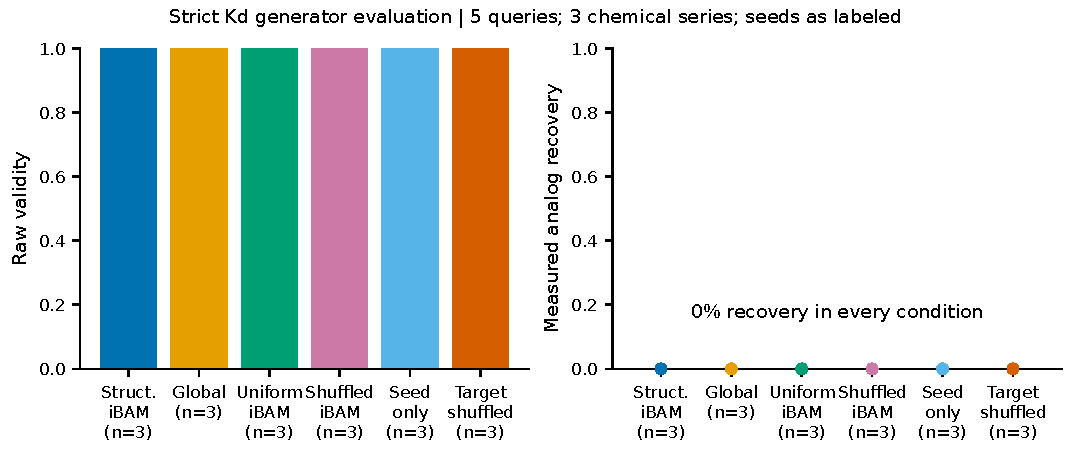
\includegraphics[width=\linewidth,height=.65\textheight,keepaspectratio]{figures/Supplementary_Figure_5_generator.pdf}
\caption{Generator outcomes across conditioning controls. Six conditioning conditions each use three training seeds and 100 draws per query across five strict Kd queries from three chemical series, totaling 9000 draws. Bars show raw validity without repair; markers show measured-analog recovery. Every condition reached full validity and zero recovery in this subset. These outcomes distinguish valid molecular graphs from recovery of measured analogs. Broader endpoint results are reported separately.}
\end{figure}
\begin{figure}[htbp]\centering
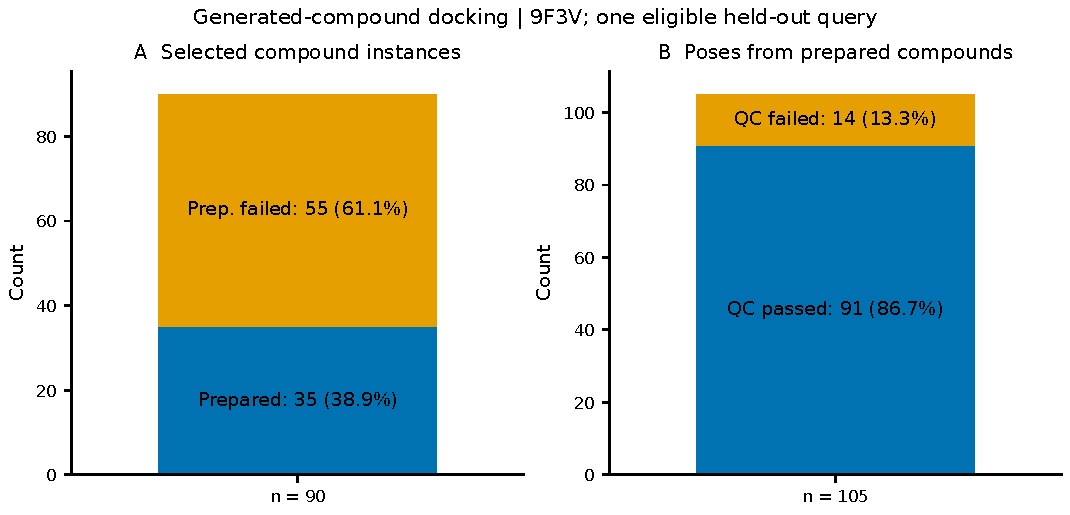
\includegraphics[width=\linewidth,height=.65\textheight,keepaspectratio]{figures/Supplementary_Figure_6_generated_docking.pdf}
\caption{Generated-compound preparation and pose checks. The analysis covers one eligible held-out query associated with receptor 9F3V. Panel A counts 90 hash-selected compound instances: 55 failed preparation and 35 were prepared. Panel B counts 105 repeated-search poses from those 35 instances: 91 passed overall PoseBusters checks and 14 failed. Preparation success is 38.9\% of selected instances; the 86.7\% pose-QC rate is conditional on preparation. Repeated poses are not independent compounds, and neither docking nor geometry checks establish binding.}
\end{figure}
\section*{Scope of the reported study}
Affinity prediction comparisons are restricted to the completed Davis warm, cold-drug, and cold-protein experiments. Architecture selection was replicated across three seeds on official validation fold 0; additional-fold selection stability was not assessed. No independent-dataset tests or local reruns of external DTA models or classical baselines are reported. Supporting screening, structural, and molecular-editing analyses retain their declared data sources and endpoint strata. Separate unfinished training was discontinued and its checkpoints remain archived outside this manuscript's evidence set.

\begin{thebibliography}{99}
\bibitem{davis2011} Davis MI, Hunt JP, Herrgard S, Ciceri P, Wodicka LM, Pallares G, et al. Comprehensive analysis of kinase inhibitor selectivity. Nat Biotechnol. 2011;29(11):1046-1051. doi:10.1038/nbt.1990.

\bibitem{deepdta2018} Öztürk H, Özgür A, Ozkirimli E. DeepDTA: deep drug-target binding affinity prediction. Bioinformatics. 2018;34(17):i821-i829. doi:10.1093/bioinformatics/bty593.

\bibitem{widedta2019} Ozturk H, Ozkirimli E, Ozgur A. WideDTA: prediction of drug-target binding affinity. 2019. doi:10.48550/arXiv.1902.04166. Preprint, arXiv:1902.04166.

\bibitem{graphdta2021} Nguyen T, Le H, Quinn TP, Nguyen T, Le TD, Venkatesh S. GraphDTA: predicting drug-target binding affinity with graph neural networks. Bioinformatics. 2021;37(8):1140-1147. doi:10.1093/bioinformatics/btaa921.

\bibitem{dgraph2020} Jiang M, Li Z, Zhang S, Wang S, Wang X, Yuan Q, et al. Drug-target affinity prediction using graph neural network and contact maps. RSC Adv. 2020;10(35):20701-20712. doi:10.1039/d0ra02297g.

\bibitem{mgraph2022} Yang Z, Zhong W, Zhao L, Yu-Chian Chen C. MGraphDTA: deep multiscale graph neural network for explainable drug-target binding affinity prediction. Chem Sci. 2022;13(3):816-833. doi:10.1039/d1sc05180f.

\bibitem{fusion2022} Yuan W, Chen G, Chen CYC. FusionDTA: attention-based feature polymerizer and knowledge distillation for drug-target binding affinity prediction. Brief Bioinform. 2022;23:bbab506. doi:10.1093/bib/bbab506.

\bibitem{ssm2023} Pei Q, Wu L, Zhu J, Xia Y, Xie S, Qin T, et al. Breaking the barriers of data scarcity in drug-target affinity prediction. Brief Bioinform. 2023;24:bbad386. doi:10.1093/bib/bbad386.

\bibitem{nhgnn2023} He H, Chen G, Chen CYC. NHGNN-DTA: a node-adaptive hybrid graph neural network for interpretable drug-target binding affinity prediction. Bioinformatics. 2023;39:btad355. doi:10.1093/bioinformatics/btad355.

\bibitem{hgtdp2024} Xiao X, Wang W, Xie J, Zhu L, Chen G, Li Z, et al. HGTDP-DTA: Hybrid Graph-Transformer with Dynamic Prompt for Drug-Target Binding Affinity Prediction. 2024. doi:10.48550/arXiv.2406.17697. Preprint, arXiv:2406.17697.

\bibitem{hcaf2025} Li J, Yao L. HCAF-DTA: drug-target binding affinity prediction with cross-attention fused hypergraph neural networks. 2025. doi:10.48550/arXiv.2504.02014. Preprint version reviewed, arXiv:2504.02014v1.

\bibitem{curvflow2026} Ma J, Yang Y, Zhao J, Zhao L. CurvFlow-DTA: dual-graph discrete Ricci curvature flow for drug-target affinity prediction. 2026. doi:10.48550/arXiv.2609.22862. Preprint, arXiv:2609.22862v1.

\bibitem{esmc2024} EvolutionaryScale. ESM Cambrian: Revealing the mysteries of proteins with unsupervised learning. 2024. \url{https://www.evolutionaryscale.ai/blog/esm-cambrian}. Accessed 24 October 2026.

\bibitem{esmcode} EvolutionaryScale. ESM software repository. 2024. \url{https://github.com/evolutionaryscale/esm}. Pinned revision fcc9d36f5fff97d9bb69a36e3252de61cc78c968; accessed 24 October 2026.

\bibitem{light2023} Li H, Zhang R, Min Y, Ma D, Zhao D, Zeng J. A knowledge-guided pre-training framework for improving molecular representation learning. Nat Commun. 2023;14:7568. doi:10.1038/s41467-023-43214-1.

\bibitem{conplex2023} Singh R, Sledzieski S, Bryson B, Cowen L, Berger B. Contrastive learning in protein language space predicts interactions between drugs and protein targets. Proc Natl Acad Sci U S A. 2023;120:e2220778120. doi:10.1073/pnas.2220778120.

\bibitem{attention2019} Jain S, Wallace BC. Attention is not Explanation. Proceedings of the 2019 Conference of the North American Chapter of the Association for Computational Linguistics: Human Language Technologies, Volume 1 (Long and Short Papers). 2019:3543-3556. doi:10.18653/v1/n19-1357.

\bibitem{sanity2018} Adebayo J, Gilmer J, Muelly M, Goodfellow I, Hardt M, Kim B. Sanity Checks for Saliency Maps. Advances in Neural Information Processing Systems. 2018. \url{https://papers.nips.cc/paper_files/paper/2018/hash/294a8ed24b1ad22ec2e7efea049b8737-Abstract.html}.

\bibitem{deepdtagen2025} Shah PM, Zhu H, Lu Z, Wang K, Tang J, Li M. DeepDTAGen: a multitask deep learning framework for drug-target affinity prediction and target-aware drugs generation. Nat Commun. 2025;16:5021. doi:10.1038/s41467-025-59917-6.

\bibitem{ho2020} Ho J, Jain A, Abbeel P. Denoising Diffusion Probabilistic Models. Advances in Neural Information Processing Systems. 2020. \url{https://arxiv.org/abs/2006.11239}.

\bibitem{discrete2021} Austin J, Johnson DD, Ho J, Tarlow D, van den Berg R. Structured Denoising Diffusion Models in Discrete State-Spaces. Advances in Neural Information Processing Systems. 2021. \url{https://arxiv.org/abs/2107.03006}.

\bibitem{morgan2010} Rogers D, Hahn M. Extended-Connectivity Fingerprints. J Chem Inf Model. 2010;50(5):742-754. doi:10.1021/ci100050t.

\bibitem{bindingdb2007} Liu T, Lin Y, Wen X, Jorissen RN, Gilson MK. BindingDB: a web-accessible database of experimentally determined protein-ligand binding affinities. Nucleic Acids Res. 2007;35(Database):D198-D201. doi:10.1093/nar/gkl999.

\bibitem{bemis1996} Bemis GW, Murcko MA. The Properties of Known Drugs. 1. Molecular Frameworks. J Med Chem. 1996;39(15):2887-2893. doi:10.1021/jm9602928.

\bibitem{vina2021} Eberhardt J, Santos-Martins D, Tillack AF, Forli S. AutoDock Vina 1.2.0: New Docking Methods, Expanded Force Field, and Python Bindings. J Chem Inf Model. 2021;61(8):3891-3898. doi:10.1021/acs.jcim.1c00203.

\bibitem{meeko} Forli laboratory. Meeko ligand preparation toolkit. 2026. \url{https://github.com/forlilab/Meeko}. Version 0.8.0; accessed 24 October 2026.

\bibitem{posebusters2024} Buttenschoen M, Morris GM, Deane CM. PoseBusters: AI-based docking methods fail to generate physically valid poses or generalise to novel sequences. Chem Sci. 2024;15(9):3130-3139. doi:10.1039/d3sc04185a.

\bibitem{pdb2000} Berman HM. The Protein Data Bank. Nucleic Acids Res. 2000;28(1):235-242. doi:10.1093/nar/28.1.235.

\bibitem{pdb6yoj} Worldwide Protein Data Bank. PDB structure 6YOJ. 2020. doi:10.2210/pdb6YOJ/pdb. FAK1-P4N complex; accessed 24 October 2026.

\bibitem{rdkit} RDKit contributors. RDKit Open source cheminformatics. 2026. \url{https://www.rdkit.org}. Version recorded in the reproducibility supplement; accessed 24 October 2026.

\bibitem{mfr2023} Hua Y, Song X, Feng Z, Wu X. MFR-DTA: a multi-functional and robust model for predicting drug-target binding affinity and region. Bioinformatics. 2023;39:btad056. doi:10.1093/bioinformatics/btad056.

\bibitem{mdf2024} Ranjan A, Bess A, Alvin C, Mukhopadhyay S. MDF-DTA: A Multi-Dimensional Fusion Approach for Drug-Target Binding Affinity Prediction. J Chem Inf Model. 2024;64(13):4980-4990. doi:10.1021/acs.jcim.4c00310.

\bibitem{prosmith2024} Kroll A, Ranjan S, Lercher MJ. A multimodal Transformer Network for protein-small molecule interactions enhances predictions of kinase inhibition and enzyme-substrate relationships. PLOS Computational Biology. 2024;20(5):e1012100. doi:10.1371/journal.pcbi.1012100.
\end{thebibliography}\end{document}